\documentclass{article}[18pt]
\usepackage{../../../../format}
\lhead{A Level Maths - M2}

\begin{document}
\begin{center}
\underline{\huge Centres of mass}
\end{center}
\begin{obeylines}
\section{Centre of mass of a discrete mass distribution}
$\bar{x}=\dfrac{\Sigma m_ix_i}{\Sigma m_i}$\\
$\bar{y}=\dfrac{\Sigma m_iy_i}{\Sigma m_i}$\\
\textbf{Example}\\
\end{obeylines}
\begin{tabular}{|c|c|c|c|}
 \hline
 Mass&$2$&$3$&$2$\\
 \hline
 $x$&2&3&-3\\
 \hline
 $y$&3&6&2\\
 \hline

\end{tabular}
\\
\\
\begin{obeylines}
$\bar{x}=\dfrac{2\times 2+3\times3+2\times-3}{2+3+2}=1$
$\bar{y}=\dfrac{2\times3+3\times6+2\times2}{2+3+2}=4$
\section{Uniform laminae}
For a triangular lamina the centre of mass is $\frac{2}{3}$ along the line from the vertex to the middle of the line opposite.
For a sector of a circle, radius r, where the angle at the centre is $2\alpha$ the centre of mass is $\dfrac{2r\sin\alpha}{3\alpha}$
\section{Rods}
In a circular arc, radius r, where the angle at the centre is $2\alpha$, the centre of mass is $\dfrac{r\sin\alpha}{\alpha}$ away from the centre.
\section{Equilibrium}
To avoid tipping, the line of action of the weight must be within the side of the lamina in contact with the plane.
If a lamina is suspended from a fixed point, the centre of mass will be vertically below the point of suspension.
Assumptions made in equilibrium calculations:
\begin{itemize}
\item No friction at the point of suspension
\item The mass of each area is uniform
\item The mass is uniform at the join
\end{itemize}



\end{obeylines}
\newpage
\begin{center}
\underline{\huge Centres of mass example - Equilibrium problems}
\end{center}
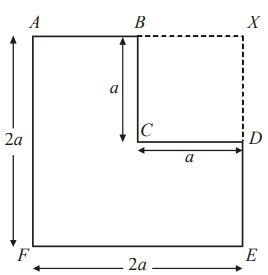
\includegraphics[width=1.5in]{eq.jpg}\\
\\
\textit{(a) Find the distance of the centre of mass of the lamina from AF. }\\

\textbf{1. Find the masses and locations of all areas or rods and put in a table}\\
\\
{\renewcommand{\arraystretch}{1.5}
\begin{tabularx}{\textwidth}{|X|X|X|}
\hline
Mass(m)&$4a^2$&$-a^2$\\
\hline
Distance From AF(x)&$a$&$\frac{3}{2}a$\\
\hline
mx&$4a^3$&$-\frac{3}{2}a^3$\\
\hline
\end{tabularx}}
\\
\\
\textbf{2. Use the formula to find the centre of mass}\\
\\
\textcolor{red}{$\bar{x}=\dfrac{\Sigma m_ix_i}{\Sigma m_i}$}\\
\\
$\bar{x}=\dfrac{\frac{5}{2}a^3}{3a^2}=\dfrac{5a}{6}$\\
\\
\textit{The lamina is freely suspended from A and hangs in equilibrium.}\\
\textit{(b) Find, in degrees to one decimal place, the angle which AF makes with the vertical.}\\
\\
\textbf{3. Use symmetry to find the y coordinate of the centre of mass}\\
\\
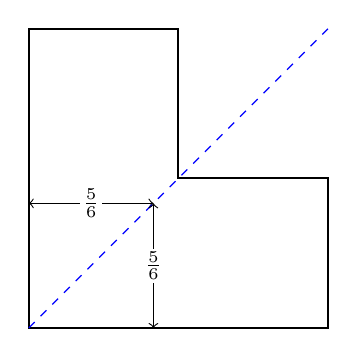
\begin{tikzpicture}[scale=1.9]
\tikzstyle{ann} = [fill=white,font=\footnotesize,inner sep=1pt]

\draw[black, thick] (0,0) -- (0,2) -- (1,2) -- (1,1) -- (2,1) -- (2,0) -- cycle;
\draw[arrows=<->](0,5/6)--(5/6,5/6);
\node[ann] at (5/12,5/6) {$\frac{5}{6}$};
\draw [blue,dashed] (0,0) -- (2,2);
\draw[arrows=<->](5/6,0)--(5/6,5/6);
\node[ann] at (5/6,5/12) {$\frac{5}{6}$};
\end{tikzpicture}
\\
\\
\textbf{4. Re-draw to find angle}\\
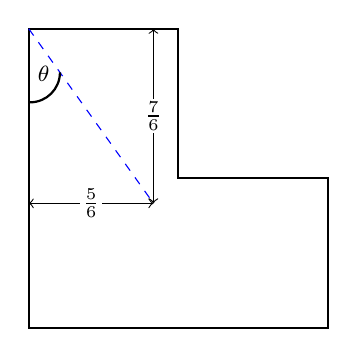
\begin{tikzpicture}[scale=1.9]
\tikzstyle{ann} = [fill=white,font=\footnotesize,inner sep=1pt]
\tikzstyle{angle} = [fill=none,font=\tiny,inner sep=1pt]
\draw[black, thick] (0,0) -- (0,2) -- (1,2) -- (1,1) -- (2,1) -- (2,0) -- cycle;
\draw[arrows=<->](0,5/6)--(5/6,5/6);
\node[ann] at (5/12,5/6) {$\frac{5}{6}$};
\draw[arrows=<->](5/6,5/6) -- (5/6,2);
\node[ann] at (5/6,17/12) {$\frac{7}{6}$};
\draw [blue,dashed] (0,2) -- (5/6,5/6);
\draw[thick] (5/24,41/24) arc (0:-90:0.2);
\node[ann] at (0.1,1.7) {$\theta$};
\end{tikzpicture}\\
\\
$\tan(\theta)=\dfrac{5/6}{7/6}$\\
\\
$\theta=35.5\degree$
\newpage




\end{document}